\newcommand{\SoftName}{GMemorise}
\newcommand{\HRule}{\rule{\linewidth}{0.5mm}}

\documentclass[a4paper]{article}
\usepackage[pdftex]{graphicx}
\usepackage{float}

\title{Measuring the Effectiveness of a Subset of Game Mechanics on Rote Memorisation of Vocabulary in the Study of a Foreign Language}
\date{30 March, 2012}
\author{Jordan West}

\begin{document}

% \maketitle
\begin{titlepage}

\begin{center}


% Upper part of the page

\includegraphics[width=0.8\textwidth]{./uqlogo.jpg}\\[1cm]    

\textsc{\Large Undergraduate Engineering Honours Thesis}\\[0.5cm]

\textsc{\LARGE Proposal}\\[0.5cm]


% Title
\HRule \\[0.4cm]
{ \Large \bfseries Measuring the Effectiveness of a Subset of Game Mechanics on Rote Memorisation of Foreign Vocabulary}\\[0.4cm]

\HRule \\[1.5cm]

% Author and supervisor
\begin{minipage}{0.4\textwidth}
\begin{flushleft} \large
\emph{Author:}\\
Jordan \textsc{West}
\end{flushleft}
\end{minipage}
\begin{minipage}{0.4\textwidth}
\begin{flushright} \large
\emph{Supervisor:} \\
Dr.~Mark \textsc{Schulz}
\end{flushright}
\end{minipage}

\vfill

% Bottom of the page
{\large \today}

\end{center}

\end{titlepage}


\tableofcontents
\newpage

\section{Introduction}
The recent proliferation of addictive game-like features (or \textit{game mechanics}) to 
increase user engagement in non-game environments such as social networks and 
sales websites raises the question: 
How effective could game mechanics be when applied in other environments, such as 
education? This project aims to construct software and analyse and quantify the
effectiveness of the application of a subset of game mechanics to an online 
learning environment in motivating and engaging students. Specifically for 
this project the learning environment selected is the memorisation of vocabulary 
of a foreign language.


% TOPIC DEFINITION %
\section{Topic Definition}
\subsection{Background} \label{background}
\subsubsection{Game Mechanics} \label{background_gamemechanics}
\subsubsection{Extrinsic vs. Intrinsic Motivation}
Motivation is often seperated into two categories - Extrinsic and Intrinsic motivation. Intrinsic motivation refers to the motivation one feels for a task when that person feels that completing the task is enjoyable or fulfilling. Extrinsic motivation 
\subsubsection{socialPsych}
The socialPsych\cite{landers_casual_2011} project examined some game mechanics
in an online social learning environment which was run in parallel to university
courses. The authors of the project compiled a list of best practices
for casual social games used for learning, of which a few are relevant to
the project discussed in this proposal. Immediacy of feedback (in terms of
rewards or validation for completing a task) was found to be important for
motivation \cite[p. 419]{landers_casual_2011}. Game rewards should also be adjusted
to a difficulty which is achievable without being overly easy to ensure the user
feels satisfaction upon completion \cite[p. 420]{landers_casual_2011}.

\subsection{Purpose}
The purpose of the project is to measure the effectiveness of applying a
subset of game mechanics to rote memorisation tasks in the study of vocabulary
in a language. By building software for this purpose, the author aims to gather
data which can quantitatively compare two otherwise identical environments 
- one which includes the selected game mechanics and one which does 
not - in terms of user engagement.

Further, the purpose is not to create a `game' as such, but rather to take some
of the components of games which are believed to make games addictive and to apply
them to a learning activity - in this case rote memorisation. The determination
of what constitutes a `game mechanic' is debatable and a
somewhat subjective topic, however for this study the game mechanics selected
have been used in many systems to date (see section \ref{background_gamemechanics}).

\subsection{Motivations}
With the success of companies such as Foursquare attributed to their game-like
features, it is difficult to determine to what extent the game-like features
have in fact contributed to their success. This project was conceived in the
hope to provide a comparison between two environments and provide a somewhat
quantitative analysis of the effectiveness of the game-like features. In
particular, whether the use of such game mechanics could be used in positive
environments such as education.

\subsection{Method}
The system will be deployed for use by students enrolled in a Japanese course at
The University of Queensland.

Users will be randomly assigned to one of two groups - Group A or Group B. Group
A will use a learning environment with a series of learning modules and tests,
while Group B will use the same learning environment with the addition of some 
game mechanics. At no point will users be required to carry out any task for
assessment or otherwise, and users may opt-out and delete all their data at
any time.

The actions of the students will be logged over a six-week period during which
the system will be available to them. Specifically which actions will be logged
is discussed in section \ref{scope_datacollection}. These actions will be 
analysed to determine the engagement of the users in each group.

\subsection{Hypothesis}
It is expected that the users of the learning environment with game mechanics applied
will display the following attributes compared to the other users:
\begin{enumerate}
	\item Using the system more often and for longer periods of time
	\item Perservering more after failed attempts at challenges
	\item Taking part in optional challenges more often
	\item Progressing through the list of challenges more quickly
\end{enumerate}


% PROJECT PLAN %
\section{Project Plan}
\subsection{Scope}
\subsubsection{Platform}
The software will be a browser based web application. This option was selected
for several reasons:
\begin{itemize}
	\item Students can easily access the software from anywhere without the
		need to install anything
	\item Bugs can be fixed extremely quickly without requiring users to
		upgrade their software
	\item All activity can be logged and stored on the server as the user
		interacts with the application, no data will not be lost if the user 
		is offline.
	\item Web applications are cross-platform.
	\item Web applications are generally faster to develop.
\end{itemize}

\subsubsection{Features}
\paragraph{Modules}
The software will provide `modules' which each contain some vocabulary to be learned.
The module order will correspond with the order in which the vocabulary should
be learned during semester. Each module will contain three challenges:
\begin{enumerate}
	\item Vocabulary List - Displays a list of vocabulary for the user to scan
		over and memorise.
	\item Test - Test the user on their knowledge of all the vocabulary for
		that module.
	\item Review - Test the user on a random selection of vocabulary from that
		module and all previous modules.
\end{enumerate}

It is expected that three modules will be completed each week for the six week
duration of the project for a total of 18 modules. It will not be explicitly
mentioned to the students that they should complete three modules per week,
however some might work this out on their own accord.
The key reason for this is that by allowing autonomy, students do not feel 
pressured into completing the challenges and believe they are completing them 
by their own will - an important defining feature of `play' vs `work'\cite{sebastian_deterding_meaningful_2011}.

\paragraph{Challenges}
For each module, three challenges will be available as discussed in the section
above. However, the availability of the challenges will be dependant upon the
group the user is assigned to. Group A (control) will have access to all
challenges at all levels from the beginning of the project. Group B will have
access only to the challenges on the first module. By completing the \textit{Test}
challenge, the following level will be unlocked. This game mechanic instills
a sense of \textit{achievement} in the student, encouraging them to unlock further
challenges \cite{gabe_zichermann_fun_2010}.


\begin{figure}[H]
	\centering
		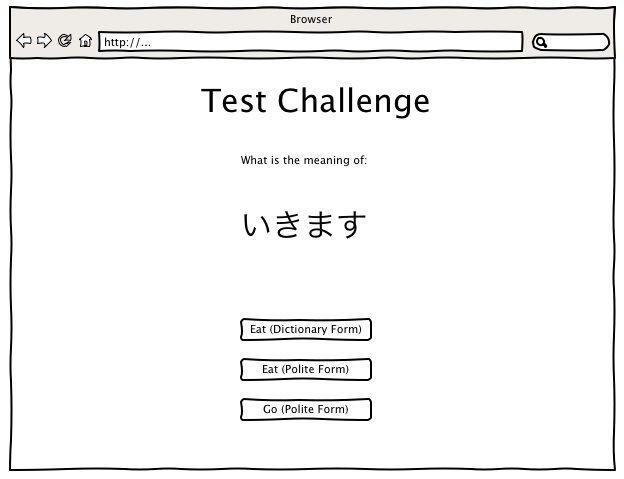
\includegraphics[width=10cm]{./screens/challenge.jpg}\\
		\caption{Mockup of a screen showing a challenge in progress}
\end{figure}

\paragraph{Points}
(Applies to Group B only)

Completing some challenges will earn the user points. The number of points earned is
dependant upon the module to which the challenge belongs, where increasing modules
result in more points earned. The Vocabulary List challenge will earn no points,
and is only available for the purpose of memorising for the Test challenge. The
Test challenge will earn the user points when it is completed the first time only
for each module. However completing the Test challenge will unlock the Review
challenge which the user can complete as many times as they wish, each time earning
points. Once the Review challenge has been completed successfully, the user must
wait 4 hours before attempting again to avoid misuse.


\begin{figure}[H]
	\centering
		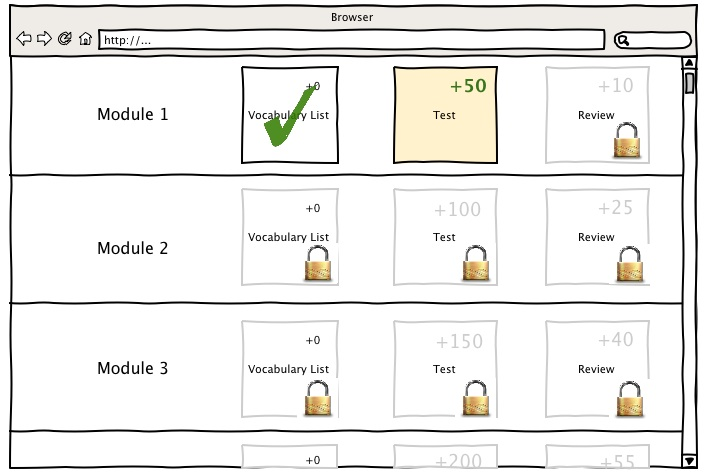
\includegraphics[width=10cm]{./screens/modules.jpg}\\
		\caption{Mockup of the list of available modules with associated challenges}
\end{figure}

\paragraph{Leaderboard}
(Applies to Group B only)
The leaderboard displays other users with a similar number of points and shows
the user how they can overtake the user above them by completing another
challenge. All users are given a ranking within the system based on their
number of points, however users can only see the ranking of other users within
three ranks of their own. This avoids leaving users feeling disappointed with
their current position and instead presents to them an achievable goal - that is to
overtake the user above them in ranking \cite{gabe_zichermann_fun_2010}.

\begin{figure}[H]
	\centering
		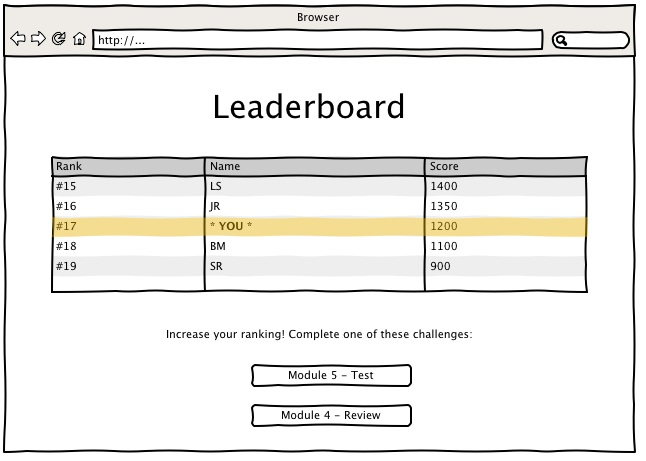
\includegraphics[width=10cm]{./screens/leaderboard.jpg}\\
		\caption{Mockup of the leaderboard showing similarly ranked users}
\end{figure}

\subsubsection{Data Collection} \label{scope_datacollection}
\paragraph{Personality Questionnaire}
During sign-up, the user will be asked to complete a short questionnaire about their personality. This questionnaire will be optional, however may provide some insights into the types of users for whom game mechanics are most effective. 

\paragraph{User Ratings}
Users will be asked to quickly rate their feelings about the system to gauge subjective feelings. To encourage users to complete the rating - this will only be asked occasionally and will be very short. The following questions will be included:

\begin{enumerate}
    \item I feel I am learning a lot with \SoftName.
    \item I look forward to using \SoftName\ each day
\end{enumerate}

The users will be asked to rate each question on a 5-point Likert scale \cite{likert_technique_1932} with the following options:
\begin{enumerate}
	\item Strongly Disagree
	\item Disagree
	\item Neither Agree nor Disagree
	\item Agree
	\item Strongly Agree
\end{enumerate}

\subsubsection{Exclusions}
The following features are beyond the scope of this project and could be examined
in future projects.

\paragraph{Scalability}
As the system is designed with a small audience in mind, it need not be capable
of handling a load of thousands of users. On a larger scale project it may be
possible to break down users into more than just two groups in order to test
many variables individually.

\paragraph{Functionality to Dynamically Add Content}
All content (vocabulary lists) will be manually added to the system. Future
modifications might allow teaching staff to add their own vocabulary to the
system to customise it for their own class.

\paragraph{Integration With Social Networks}
Another aspect of gaming which is ignored in this project is social gaming.
Adding integration with social networks such as Facebook and Twitter could add
the complex element of peer validation to the user motivation. Except for the
leaderboard competition, the social aspect of game mechanics will not be 
investigated in this project.

\subsection{Milestones}
\subsubsection{Planning and Proposal}
(5 weeks)
The initial stage is the project planning for which the deliverable is this document.

\subsubsection{Requirements}
(1 week)
Following planning, a requirements document should be prepared which details the scope of the project in more detail. This ensures a clear understanding of the technical work required to complete the project.

\subsubsection{UI Design and Layouts}
(2 Weeks)
With the requirements in place, the layout of the user interface (UI)

\subsection{Schedule}
\begin{tabular} { l | l || l }
	Week & Beginning & Task \\
	\hline
	1 - 5 & 28 Feb - 30 Mar & Project Proposal and Planning \\
	6       & 2 Apr           & Gather Project Requirements  \\
	7       & 16 Apr          & Initial UI Designs and Layouts  \\  
	8       & 23 Apr          & Contact teaching staff          \\  
	9       & 30 Apr          & Gather/create vocabulary lists  \\  
	10      & 7 May           & Coding                         \\  
	11      & 14 May          & \vdots                          \\  
	12      & 21 May          & \vdots                          \\  
	13      & 28 May          & Testing and bug fixing          \\  
	14      & 23 Jul          & Information to students and signup \\  
	15      & 30 Jul          & Data Collection Week 1          \\  
	16      & 6 Aug           & Data Collection Week 2          \\  
	17      & 13 Aug          & Data Collection Week 3          \\  
	18      & 20 Aug          & Data Collection Week 4          \\  
	19      & 27 Aug          & Data Collection Week 5          \\  
	20      & 3 Sep           & Data Collection Week 6          \\  
	21      & 10 Sep          & Analyse Results                 \\  
	22      & 17 Sep          & \vdots                          \\  
	23      & 1 Oct           & \vdots                          \\  
	24      & 8 Oct           & Compilation of Results and Report \\
	25      & 15 Oct          & \vdots                          \\  
	26      & 22 Oct          & Submit Thesis  \\  
\end{tabular}

\section{Risk Assessment}
As this project is predominantly software oriented, all design tasks will be carried
out in a low-risk laboratory.
\subsection{OH\&S risks}
\begin{tabular}{ l | l }
	Risk  &  Mitigation \\
	\hline
	\hline
	Repetitive Strain Injury or related  & Take frequent breaks from     \\
	injuries from computer usage.         & working and stretch/exercise. \\
	\hline
\end{tabular}
\subsection{Project Risks}
\begin{tabular}{ l | l }
	Risk  & Mitigation  \\
	\hline
	\hline
	Teaching staff may not wish for      & Contact teaching staff early in  \\
	their students to participate.       & semester. \\
	\hline
	Ethics Committee may not approve     & Seek Ethics Committee approval  \\
	study.                               & as early as possible.           \\
	\hline
	Users of the system may communicate     & Ask users not to discuss the system \\
	thereby invalidating the results.       & until after the 6 week data collection period.\\
	\hline
\end{tabular}

\newpage
\bibliographystyle{plain}
\bibliography{thesis}
\end{document}
